\section{Electrons}
\label{sec:el}

PFElectrons returned by the PF algorithm require further identification before being used as analysis objects. The additional selections are combined into an electron identification (ID), which discriminates isolated prompt TODO(define prompt) signal electrons from conversion electrons and PFJets TODO(dont like jets). The ID can be set for working points TODO(WP jargon?), with the tight and veto working points being shown shown in Table \ref{tb:elID}. Each of the identification cuts are explained in more detail in the following sections.

\input{Tables/Tb_ElID.tex}

\subsection{Cluster Shape $\sigma_{i\eta i\eta}$}
\label{ssec:idss}

\subsection{$|\Delta \eta_{in}|$ and $|\Delta \phi_{in}|$}


$|\Delta \eta_{in}|$ and $|\Delta \phi_{in}|$ are the absolute $\eta$ and $\phi$ differences between the SC position of the electron and the track direction at the primary vertex extrapolated to the ECAL assuming no Brehmstrahlung has occured. These cuts are used as the SC position can be biased by additional particles associated with hadron and conversion backgrounds. TODO(heavier particles bend more? more emission?) When an electron emits Brehmstrahlung radiation the $\phi$ distribution gets smeared TODO(so cuts are much hugher for phi than eta). 

TODO(what in in? is it just in? why?)


% \begin{figure}[htpb]
% 	\centering
% 	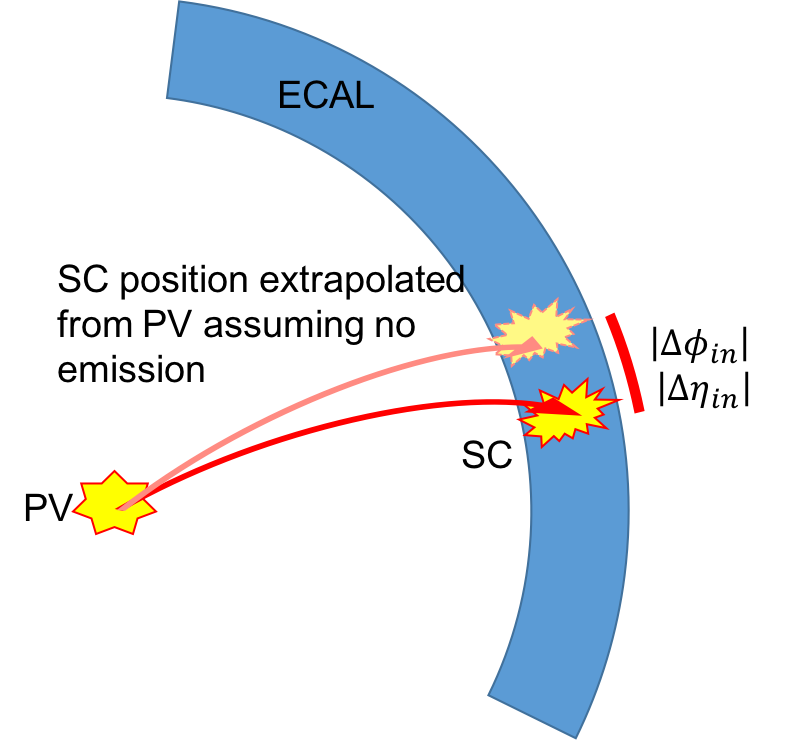
\includegraphics[width=0.4\textwidth]{Figures/deltaEtadeltaPhi}
% 	\caption[A sketch showing the electron identification variables $|\Delta \eta_{in}|$ and $|\Delta \phi_{in}|$]{ A sketch showing the electron identification variables $|\Delta \eta_{in}|$ and $|\Delta \phi_{in}|$ }
% 	\label{fig:eIDetaphi}
% \end{figure}

\subsection{$|\frac{1}{E}-\frac{1}{p}|$}
\label{ssec:id4}

\label{ssec:id2}
\subsection{$\frac{H}{E}$}
\label{ssec:id3}

\subsection{Isolation}
\label{ssec:id42}
\subsection{Missing Inner Hits and Conversion Veto}
\label{ssec:id5}
\subsection{$d_{0}$ and $d_{z}$}
\label{ssec:id6}

